\chapter{State of the Art}
\label{capitolo3}
\thispagestyle{empty}

\noindent In this chapter the main challenges of automatic sunspot detection are analysed and several state of the art algorithms that overcome these challenges are presented, together with an assessment of their advantages and disadvantages. The reader will also understand why being able to automatically segment images of the Sun and perform sunspot clustering is so critically important. \\ Manually drawing the contours of dark patches with white background can look trivial to the inexperienced eye, but centuries of disagreements among scientist on that matter demonstrated that this is actually not the case. In fact, irregularities in the shape of the sunspots and their variable intensity and contrast with the surroundings make their automated detection from digital images difficult \cite{curto2008automatic}. Similarly, automatically clustering sunspots into groups, taking into account the properties of magnetic field, has revealed itself to be a rather complex task. In the past, given the moderate quantity of data available to the scientists, it was quite easy to label all the images. During the years technological development progressively enhanced the quality of datasets at our disposal. From December 1995, when the SOHO mission was launched, the Sun has been under almost constant human surveillance from space. Since then, the space telescope has delivered a daily stream of 250MB of solar data back to researchers on Earth. With 12 instruments on board, probing every area of our star, SOHO has compiled a vast library of solar data. This solar work of art is beginning to be complemented by SDO, which is returning 1.5TB of data per day, comprising constant streams of high-resolution images of the Sun over 10 spectral channels \cite{esa-soho}. The volume of data produced by SDO has made it necessary to develop new ways of analysing it.\\
In the early stages of the development of this thesis traditional image processing appraches have been explored in order to tackle sunspot detection. Unfortunately methods like edge detection \cite{canny1987computational}, or simple segmentation algorithms like watershed transform \cite{beucher1992watershed} or histogram clustering \cite{puzicha1999histogram} are simply not powerful enough to yield acceptable performance on this task. On one hand both edge detection and watershed fail badly, tending to get confused by the noise introduced by convection cells, and ending up overdetecting. Hyperparameter tuning can possibly help in many cases but it is impossible to find the right values in order for the methods to generalize on unseen images. Even selecting ad-hoc parameters for every example the detection performance remains very poor. Such a strong evidence testifies that the above-mentioned approaches are not suitable solutions to the problem this work aims to tackle. On the other hand, even though histogram clustering is a very na\"{i}ve approach and yields poor performance on the general segmentation task, later on in this thesis it will be shown that very simple clustering algorithms are able to distinguish umbrae from penumbrae given the mask of the selected sunspot and its classification.\\
Nontheless, during the 1990s and the early 2000s, similarly simple methods were regulary employed, most of them with human supervision. At that time the existing techniques for sunspot detection could be divided into the three basic classes \cite{zharkov2004}:
\begin{itemize}
  \item \textbf{Thresholding} methods: relying on disk intensity variation;
  \item \textbf{Border} methods \cite{pettauer1997novel}: using the gradient of the intensity of the image;
  \item \textbf{Bayesian Pattern Recognition} methods \cite{turmon2002statistical}: applying simple statistical analysis to data labeled with expert identification or unsupervised clustering.
\end{itemize}
In addition to being far from autonomous, all these methods are data specific, in the sense that they were developed for specific datasets and, hence, make a number of assumptions about the properties of the data, image resolution, average intensity and presence of image artefacts \cite{zharkov2004}.\\
Around 2010, probably driven by the launch of SDO (February 11, 2010), automatic solar feature analysis saw a new wave of research, with novel, far more complex methods being published. The ones that had greater impact in the field are the following \cite{verbeeck2013multi}: the \textbf{Automated Solar Activity Prediction (ASAP)} and the \textbf{Sunspot Tracking And Recognition Algorithm (STARA)} \cite{watson2009modelling} that detect sunspots in white-light continuum images; the \textbf{Spatial Possibilistic Clustering Algorithm (SPoCA)}  \cite{barra2009fast} that automatically segments solar EUV images into active regions, coronal holes and quiet Sun  and the \textbf{Solar Monitor Active Region Tracker (SMART)} \cite{higgins2011solar} that detects active regions in line-of-sight magnetograms. The ones that are most relevant with respect to the work that will be presented in the next chapters are definitely ASAP and STARA, since they both use data in the same spectrum band (white-light) as our algorithm. However, a direct comparison would not be fair, because they also use other wavelengths in addition to the one in common.\\
ASAP is actually a set of algorithms for sunspot, faculae, and active-region detections \cite{colak2008automated} and solar-flare prediction \cite{colak2009automated}. Many versions of this tool exist, the one that best relates to this thesis  was published in 2011 \cite{colak2011representation}. This more recent version uses both continuum intensitygrams and magnetograms (SOHO/MDI) to produce segmented groups of sunspots while previous works also asked for quick look (in GIF or JPEG format) images as input for its processes. The main steps in this algorithm can be summarized as follows:
\begin{enumerate}
  \item Pre-procesing to detect the solar disk and remove limb darkening;
  \item Coordinate conversion: detected solar disks are converted from heliocentric coordinates to Carrington heliographic coordinates (see the glossary in Appendix1 for to find information on this matter or refer to \textit{Coordinate systems for solar image data} \cite{thompson2006coordinate} manual).
  \item intensity filtering threshold value $T = \mu - (\sigma \times \alpha)$ is applied where $\mu$ is the mean, $\sigma$ is the standard deviation of the image, and $\alpha$ is a constant.
\end{enumerate}
\begin{figure}[t]
    \centering
    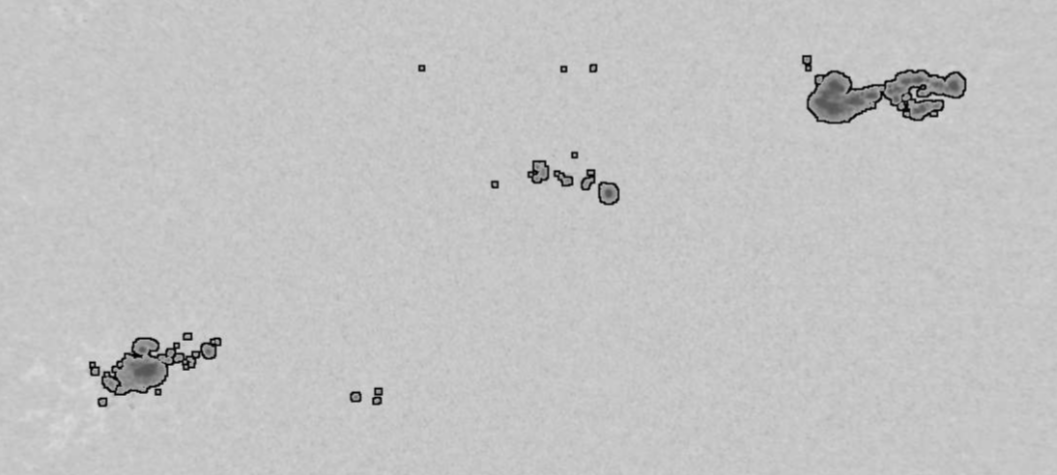
\includegraphics[width=\textwidth]{./pictures/asap-example-detection}
    \caption{An example of ASAP detections from 10 June 2003.}
    \label{fig:asap-example}
\end{figure}
In practice ASAP works pretty well \cite{verbeeck2013multi} although the coordinate system change shows advantages and disadvantages. The main advantage is that towards the limb of the Sun on a two dimensional heliocentric image each degree will be represented by fewer pixels while in a heliographic image each degree is represented with same amount of pixels. Ideally, this trick corrects the distortions due to perspective on the original data and relieves the subsequent pipeline of models from the burden of dealing with it. Although coordinate conversion sounds like a very sensible approach, it actually introduces a bias in the produced image, because it needs to interpolate neighbouring pixels when the mapping is not one to one. Also, the main problem with this approach is represented by the fact that the transformation is computationally expensive. For instance, the application on ASAP to SDO/HMI \cite{schou2012design} images larger than 1024 by 1024 pixels shows that heliographic conversion algorithms must, in some way, be made more efficient to tackle larger images \cite{verbeeck2013multi}. Also, like every other method that that employs thresholding it is hardly generalizable on heterogeneous data and inherently less tolerant to noise. In any case, ASAP has been developed to work on images belonging to a well-established dataset produced by SOHO space telescope. This ensures an homogenous data distribution and a really low noise level (compared to telescopes observing from underneath the atmosphere of the Earth). \\
\begin{figure}[t]
    \centering
    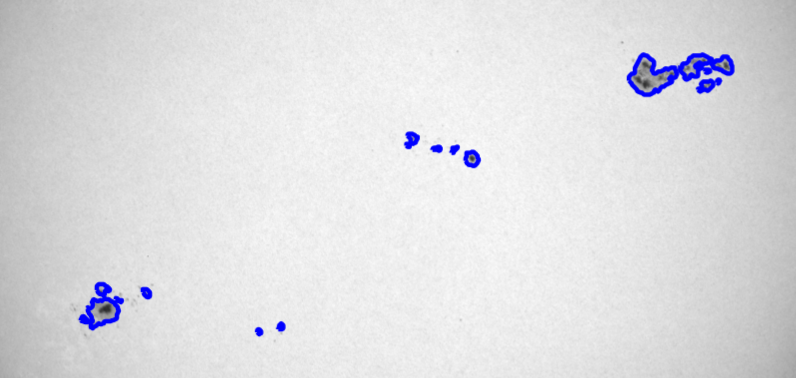
\includegraphics[width=\textwidth]{./pictures/stara-example-detection}
    \caption{An example of STARA detections from 10 June 2003.}
    \label{fig:stara-example}
\end{figure}
The STARA algorithm was originally developed to analyze the data generated by SOHO but has since been improved to be able to take advantage of the new data recorded by SDO and, unlike ASAP, several ground-based instruments \cite{ravindra2013digitized}. STARA makes use of morphological image processing techniques \cite{dougherty2003hands} to be able to efficiently process large datasets. Specifically, the images are inverted to leverage the top-hat transform that detects the intensity peaks in an image. This can be thought of as moving a circle (structuring element) underneath the profile and marking out the path of its centre. As the structuring element is chosen to be larger than the width of the sunspot peaks, it cannot fit into those peaks and so their depth is reduced. This profile is then morphologically dilated (dual transform to erosion). In formulas: $T(f) = f - ((f \ominus  s) \oplus  s)$ where $f$ is the original data, $\ominus$ is the erosion operation, $\oplus$ is the dilation operation, and $s$ is the structuring element. Doing this gives a very similar profile to that of the original image, but without the sunspot peaks present. Subtracting this profile from the original yields the final sunspot candidates. In practice STARA demonstrated to work so consistently on space telescope data that NASA released a data catalogue with it and to ensure the detections were as accurate as possible a labeled dataset containing human sunspot detections was used as a ground truth in order for the optimal structuring element to be chosen. Nontheless STARA cannot yet be considered as fully autonomous when applied on ground-based telescope data. For instance, tests conducted in the Kodaikanal (India) observatory showed that human intervention is still needed in some cases \cite{ravindra2013digitized}. Also, STARA is not able to perform sunspot clustering. Once it detects where the interesting features are located in the image it needs to be complemented by other algorithms like SPoCA or SMART to be able to partition the sunspots into groups.\\
Similar algorithms using mathematical morphology for image segmentation have been applied to data coming from ground observatories. An exaple is the pipeline that was set-up at the Ebro Observatory \cite{ebro-observatory} located in Spain. It uses the top-hat transform to detect sunspots and then apply a threshold on the heliographic distance among them for grouping \cite{curto2003automatic}. Accorrding to their statistics, the sunspots neighboring scale is 6 heliographic
degrees, this means that sunspots which are separated less than $6\degree$ are part of the same solar group. This is a very simple method that works in some cases but still when groups are placed in a very close space, mostly in the maximum of the solar cycle, the operators who supervises the whole process at Ebro must manually redefine the classification \cite{curto2003automatic}. \\
More recent attempts to tackle the problem of sunspot detection and clustering are not well documented and it seems the research field has reached a plateau during the last years. Most ground-based observatories are using combinations of the simple methods described above and human supervision \cite{pucha2016development}. Nontheless, until now, we are still very far away from having an autonomous agent that is able to accurately estimate the number of sunspots without external intervention. However, in this thesis we show that this is actually possible using modern Computer Vision techinques, like Deep Learning. \\
It is not the first time that advanced statistics is being utilized to study or predict the behaviour of the Sun. Around 2005, simple Machine Learning approaches have been explored for sunspot classification \cite{colak2007automatic}\cite{nguyen2006learning}\cite{nguyen2005rough}. They mainly used decision trees on hand-crafted features in order to be able to predict the McIntosh class of a group of sunspots. More recently, with the raise of Deep Learning, deep neural networks started to be employed for space weather prediction, in particular to perform forecasting on solar flares, solar energetic particles, and coronal mass ejections. So many studies have been published on this multi-disciplinary research field that NASA's 2017 Frontier Development Laboratory decided to develop FlareNet \cite{McGregor2017}, a software framework for experimentation within these problems. FlareNet includes components for the downloading and management of SDO data, visualization, and rapid prototyping. The system architecture is built to enable collaboration between heliophysicists and machine learning researchers on the topics of image regression, image classification, and image segmentation. \\
On this path to revolutionizing solar physics whith Artificial Intelligence, our work will be seeking to create an agent that is capable of completely replacing the human expert in the process of sunspot counting.
\begin{figure}[t]
    \centering
    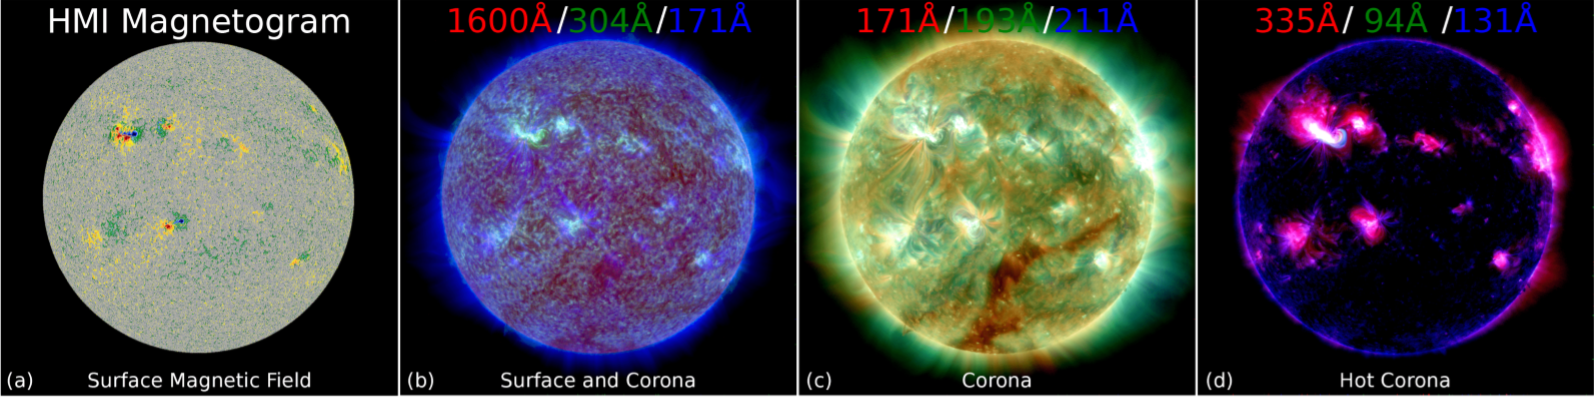
\includegraphics[width=\textwidth]{./pictures/flarenet}
    \caption{Data visulized with FlareNet: (a) The Helioseismic and Magnetic Imager (HMI) \cite{schou2012design}, colorized full-disk images of surface magnetic field; (b, c, d) The Atmospheric Imaging Assembly (AIA) \cite{lemen2011atmospheric}, 8 channels ranging from UV ro EUV composend into RGB images.}
    \label{fig:flarenet}
\end{figure}
